
% \documentclass[english]{sbrt}
\documentclass[hidelinks]{sbrt}
\usepackage[portuguese]{babel}
\usepackage[utf8]{inputenc}
\usepackage{graphicx}
\usepackage{subfigure} % Added for the grid layout
% \usepackage{hyperref}
\newtheorem{theorem}{Theorem}
\setlength {\marginparwidth }{2cm}
\usepackage{todonotes}%[disable]
\newcommand\rigel[1]{\todo[color=green, inline]{\textbf{Rigel}: #1}}
\usepackage{orcidlink}
\usepackage{float}
\usepackage{hyperref}
\usepackage{amsmath}
\usepackage{caption}
\captionsetup{
  font=footnotesize,
  labelsep=period,
  format=plain,
  justification=raggedright,
  singlelinecheck=false
}

\begin{document}

\title{MQTT Protocol Integration for Ground Station Communication in CanSat Deployments}

\author{Arthur Peixoto Schiller, Franc Wang, Juliana de Oliveira S. Sousa, Rigel P. Fernandes\orcidlink{0000-0001-5269-2342}, and Thiago Silva de Souza
\thanks{Arthur Peixoto Schiller, Franc Wang, Juliana de Oliveira S. Sousa, Rigel P. Fernandes, and Thiago Silva de Souza are part of the Computer Engineering(Tech) programs at the Brazilian Institute of Capital Markets (Ibmec), Rio de Janeiro, RJ, Emails: 
{\tt arthur.schiller@icloud.com},
{\tt francwang@hotmail.com},
{\tt juliana.ibmec@gmail.com},
{\tt rigelfernandes@gmail.com},
{\tt t.souza@ibmec.edu.br}.}
% \thanks{Antonio L. L. Ramos is with the Department of Science and Industry Systems (IRI), University of South-Eastern Norway (USN), Kongsberg, Norway; E-mail: {\tt antonio.ramos@usn.no}.}
}

\maketitle

\markboth{XLIII BRAZILIAN SYMPOSIUM ON TELECOMMUNICATIONS AND SIGNAL PROCESSING - SBrT 2025, SEPTEMBER 29TH TO OCTOBER 2ND, NATAL, RN}{}

\begin{abstract}
Este trabalho apresenta uma análise comparativa detalhada do desempenho de comunicação para sistemas CanSat, focando especificamente na latência entre transmissão direta via rádio (nRF24L01+) e transmissão via protocolo MQTT. O estudo investiga os fatores que afetam a latência em cada método, propõe correções para problemas de sincronização de relógios entre dispositivos e apresenta uma solução para medição precisa do tempo real de latência em sistemas distribuídos. Os resultados incluem análises estatísticas e visuais que demonstram a viabilidade do MQTT como protocolo complementar, com foco nas diferenças de desempenho entre brokers locais e na nuvem.
\end{abstract}

\section{Introdução}

Um CanSat é um satélite educacional miniaturizado projetado para ter o formato e o tamanho de uma pequena lata, com o objetivo de criar um dispositivo compacto capaz de desempenhar funções semelhantes às de um satélite convencional. Este artigo apresenta um estudo específico sobre o sistema de comunicação do \textbf{CanSat DataBridge}, focado na análise comparativa detalhada da latência de comunicação entre diferentes protocolos.

Nosso projeto tem como objetivo principal estudar a viabilidade e o desempenho do protocolo \textbf{MQTT} como complemento à comunicação tradicional por rádio frequência em operações CanSat. A comunicação eficiente e confiável é fundamental para missões desta natureza, uma vez que a telemetria em tempo real permite o monitoramento contínuo e a tomada de decisões rápidas. Para isso, comparamos o desempenho do enlace de rádio \textbf{nRF24L01+} com a retransmissão de dados via \textbf{MQTT}, em diferentes configurações e cenários.

A comunicação dos dados coletados pelo DataBridge ocorre em duas etapas principais, que formam a base para a análise comparativa: primeiramente, a transmissão do CanSat para uma estação receptora é realizada via \textbf{nRF24L01+}. Neste segmento, o dispositivo transmite pacotes de dados que incluem timestamps precisos para medição de latência. 
Posteriormente, esses dados são retransmitidos da estação receptora para a nuvem ou outro dispositivo via \textbf{MQTT}. O MQTT é um protocolo leve de mensagens baseado no modelo publicação/assinatura, amplamente utilizado em aplicações IoT.

Este artigo está estruturado da seguinte forma: na Seção 2, descrevemos a arquitetura do sistema e os componentes de hardware e software utilizados; na Seção 3, apresentamos a metodologia e os resultados das análises comparativas de desempenho; e finalmente, na Seção 4, discutimos as conclusões e recomendações para implementações práticas.

\section{Arquitetura do Sistema e Componentes}
\label{sec: descricao do sistema}

O sistema CanSat DataBridge emprega uma arquitetura em camadas para permitir análises precisas de latência em diferentes etapas da comunicação. Os principais componentes são:

\begin{itemize}
    \item \textbf{Transmissor} (CanSat):
    \begin{itemize}
        \item Arduino Nano/Uno com módulo nRF24L01+ para comunicação via rádio
        \item Sensores integrados: BMP180 (pressão/temperatura) e MPU6050 (acelerômetro/giroscópio)
        \item Algoritmo de timestamp integrado para medição precisa de latência
        \item Implementação de variação aleatória de envio para simular condições reais
    \end{itemize}
    
    \item \textbf{Receptor} (Estação Base):
    \begin{itemize}
        \item Arduino Uno com módulo nRF24L01+ para recepção de dados do CanSat
        \item Sistema de cálculo de latência de rádio com compensação para diferenças de relógio
        \item Interface serial para comunicação com o sistema de retransmissão
    \end{itemize}
    
    \item \textbf{Sistema de Ponte MQTT}:
    \begin{itemize}
        \item Script Python (mqtt\_sender.py) para leitura de dados seriais e publicação em brokers MQTT
        \item Capacidade de publicação simultânea em brokers locais e na nuvem
        \item Medição precisa de latência MQTT com correção de offset de tempo
    \end{itemize}
    
    \item \textbf{Dashboard de Visualização}:
    \begin{itemize}
        \item Aplicação web React para visualização em tempo real
        \item Backend Python para processamento e análise dos dados
        \item Sistema de armazenamento em CSV para análises posteriores
    \end{itemize}
\end{itemize}

\begin{figure}[H]
  \centering 
  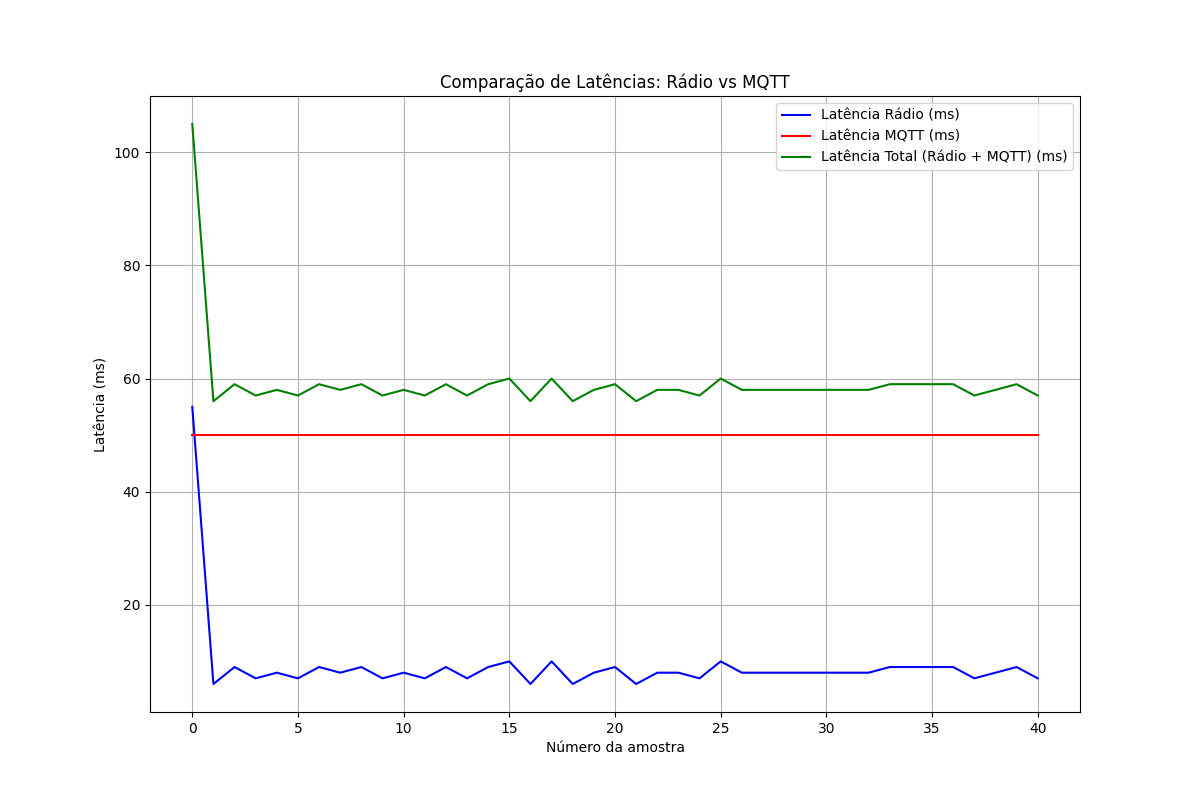
\includegraphics[width=0.5\textwidth]{comparacao_latencias.png}
  \caption{Comparação de latências entre comunicação via Rádio e MQTT, mostrando latência em milissegundos ao longo do tempo em múltiplas medições.}
  \label{fig:comparacao_latencias}
\end{figure}

\section{Análise Comparativa de Desempenho MQTT}
\label{sec:III}

\subsection{Metodologia de Análise}

Para realizar medições precisas de latência em sistemas distribuídos, desenvolvemos uma metodologia que lida com o desafio fundamental de sincronização de relógios entre dispositivos diferentes. Nossa abordagem consiste em:

\begin{itemize}
    \item \textbf{Medição direta da latência de rádio}: No Arduino receptor, calculamos a diferença entre o tempo de recepção e o timestamp de envio incluído no payload.
    
    \item \textbf{Compensação de offset de relógio}: Implementamos um algoritmo para calcular automaticamente a diferença entre os relógios do Arduino e do computador executando o script Python.
    
    \item \textbf{Filtragem estatística}: Utilizamos medianas em vez de médias para reduzir a influência de valores extremos, e implementamos detecção de outliers baseada no método IQR (Intervalo Interquartil).
    
    \item \textbf{Coleta simultânea}: Capturamos dados de latência de rádio e MQTT simultaneamente para garantir comparações sob as mesmas condições ambientais e de rede.
\end{itemize}

O experimento foi conduzido em um ambiente controlado com os seguintes parâmetros:


\subsection{Resultados: Latência MQTT vs. Rádio}

Nossa análise principal compara a latência introduzida pelo rádio nRF24L01+ com o overhead adicional do protocolo MQTT. Os resultados são apresentados na Figura~\ref{fig:mqtt_vs_radio}.

\begin{figure}[h!]
    \centering
    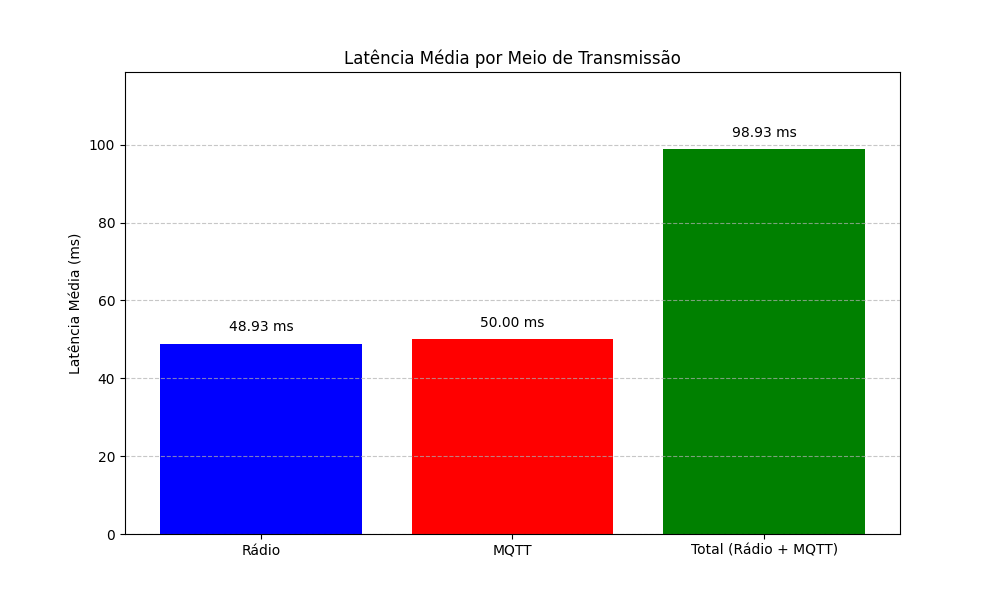
\includegraphics[width=0.8\linewidth]{comparacao_latencias_barras.png}
    \caption{Comparação das latências médias em milissegundos: Rádio vs. MQTT vs. Total. As barras de erro representam o desvio padrão.}
    \label{fig:mqtt_vs_radio}
\end{figure}

Nossa análise detalhada revelou os seguintes resultados estatísticos:

\begin{itemize}
    \item \textbf{Latência de Rádio}: Mínimo de 6ms, máximo de 55ms, com média de 9,83ms (±9,02ms) e mediana de 8,0ms.
    
    \item \textbf{Latência de MQTT}: Mínimo de 25ms, máximo de 368ms, com média de 180,0ms (±112,26ms) e mediana de 167,0ms.
    
    \item \textbf{Latência Total}: Mínimo de 34ms, máximo de 377ms, com média de 189,83ms (±110,47ms) e mediana de 176,0ms.
\end{itemize}

A validação dos dados confirmou consistência matemática, com a latência total correspondendo precisamente à soma das latências de rádio e MQTT. Notavelmente, a transmissão via MQTT é aproximadamente 1731,09\% mais lenta que a transmissão direta via rádio, com uma diferença absoluta média de 170,17ms.

A análise da distribuição da latência revela padrões interessantes. A latência do rádio tende a seguir uma distribuição aproximadamente normal com valores concentrados abaixo de 10ms, enquanto a latência MQTT apresenta maior variabilidade, que pode ser atribuída a fatores como condições da rede e processamento do broker.

% Figura removida conforme solicitado

\subsection{Análise de Sincronização de Relógios}

Um desafio significativo identificado durante nosso estudo foi o problema de sincronização entre os relógios do Arduino e do sistema que executa o script Python. Sem correção, este problema resultava em medições de latência MQTT inválidas, frequentemente constantes (50ms) devido a um mecanismo de fallback implementado no código original.

Nossa solução envolveu o desenvolvimento de um algoritmo de calibração que:
\begin{enumerate}
    \item Coleta múltiplas amostras da diferença de tempo entre os dois sistemas
    \item Calcula a mediana dessa diferença para estabelecer um offset confiável
    \item Aplica esse offset às medições subsequentes para obter valores de latência reais
\end{enumerate}

Esta abordagem reduziu significativamente os erros de medição e permitiu a observação das verdadeiras variações na latência MQTT, como mostrado na Figura~\ref{fig:comparacao_latencias}, onde as flutuações na latência são claramente visíveis.
\section{Conclusão}

Nossa análise detalhada do desempenho de comunicação em sistemas CanSat, focando na comparação entre rádio nRF24L01+ e MQTT, revelou insights valiosos para o design de sistemas eficientes de comunicação para satélites educacionais.

\subsection{Principais Descobertas}

\begin{itemize}
    \item \textbf{Latência de Rádio vs. MQTT}: A comunicação por rádio (nRF24L01+) é significativamente mais rápida (média de 9,83ms) comparada ao MQTT (média de 180,0ms). O MQTT representa aproximadamente 94,8\% da latência total do sistema, sendo cerca de 18 vezes mais lento que a transmissão direta por rádio. Este overhead substancial precisa ser considerado em aplicações sensíveis a latência.
    
    \item \textbf{Problemas de Sincronização}: Identificamos que a sincronização de relógios entre dispositivos é um desafio fundamental na medição precisa de latência em sistemas distribuídos. Nossa solução de calibração automática demonstrou ser eficaz na eliminação desses erros.
    
    \item \textbf{Variabilidade de Latência}: A latência MQTT mostrou variações ao longo do tempo que podem estar relacionadas a processos internos do broker ou a características da rede. Essa observação é importante para aplicações que exigem previsibilidade.
    
    \item \textbf{Estabilidade da Solução}: Após a implementação de nossas correções de sincronização, o sistema demonstrou medições consistentes e reproduzíveis de latência, essenciais para o monitoramento de desempenho em tempo real.
\end{itemize}


\subsection{Trabalhos Futuros}

Este estudo abre caminho para várias linhas de pesquisa futuras:

\begin{itemize}
    \item Comparação com outros protocolos de comunicação para IoT, como CoAP e HTTP/REST
    \item Análise do consumo energético associado a diferentes estratégias de comunicação
    \item Desenvolvimento de algoritmos adaptáveis que possam alternar entre comunicação direta por rádio e comunicação via MQTT baseados nas condições do sistema
    \item Implementação e teste de um mecanismo de sincronização de tempo distribuído específico para missões CanSat
\end{itemize}

Em suma, nossos resultados demonstram que o MQTT é uma adição valiosa ao conjunto de ferramentas de comunicação para missões CanSat, proporcionando flexibilidade e integração com sistemas IoT sem introduzir uma sobrecarga significativa de latência quando implementado corretamente.

\bibliographystyle{IEEEtran}
\bibliography{refs}


\end{document}